\documentclass[11pt,letterpaper]{article}
\usepackage[lmargin=1in,rmargin=1in,tmargin=1in,bmargin=1in]{geometry}
\usepackage{../style/homework}
\usepackage{../style/commands}
\setbool{quotetype}{false} % True: Side; False: Under
\setbool{hideans}{true} % Student: True; Instructor: False

% -------------------
% Content
% -------------------
\begin{document}

\homework{21: Due 12/15}{All paths are not equal; if they were, they wouldn't be paths but rather the points at each end.}{H.E. Huntley}

% Problem 1
\problem{10} Does the graph $G$ below have an Euler circuit or Euler trail? If it has an Euler circuit or Euler trail, find it. If it does not have an Euler circuit or Euler trail, explain why not. 
	\[
	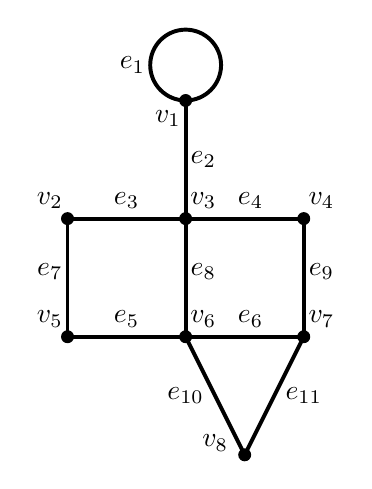
\begin{tikzpicture}[scale=1.5]
	\draw[line width=0.05cm] (0,2.3) circle (0.3);
	\draw[line width=0.05cm] (0,2) to (0,1);
	\draw[line width=0.05cm] (-1,1) to (1,1);
	\draw[line width=0.05cm] (-1,0) to (1,0);
	\draw[line width=0.05cm] (-1,1) to (-1,0);
	\draw[line width=0.05cm] (1,1) to (1,0);
	\draw[line width=0.05cm] (0,1) to (0,0);
	\draw[line width=0.05cm] (0,0) to (0.5,-1);
	\draw[line width=0.05cm] (1,0) to (0.5,-1);
	
	\draw[fill= black] (0,2) circle (0.05);
	\draw[fill= black] (-1,1) circle (0.05);
	\draw[fill= black] (0,1) circle (0.05);
	\draw[fill= black] (1,1) circle (0.05);
	\draw[fill= black] (-1,0) circle (0.05);
	\draw[fill= black] (0,0) circle (0.05);
	\draw[fill= black] (1,0) circle (0.05);
	\draw[fill= black] (0.5,-1) circle (0.05);
	
	\node at (-0.15,1.85) {$v_1$};
	\node at (-1.15,1.15) {$v_2$};
	\node at (0.15,1.15) {$v_3$};
	\node at (1.15,1.15) {$v_4$};
	\node at (-1.15,0.15) {$v_5$};
	\node at (0.15,0.15) {$v_6$};
	\node at (1.15,0.15) {$v_7$};
	\node at (0.25,-0.90) {$v_8$};

	\node at (-0.45,2.3) {$e_1$};
	\node at (0.15,1.5) {$e_2$};
	\node at (-0.5, 1.15) {$e_3$};
	\node at (0.55,1.15) {$e_4$};
	\node at (-0.5,0.15) {$e_5$};
	\node at (0.55,0.15) {$e_6$};
	\node at (-1.15,0.55) {$e_7$};
	\node at (0.15,0.55) {$e_8$};
	\node at (1.15,0.55) {$e_9$};
	\node at (0,-0.5) {$e_{10}$};
	\node at (1,-0.5) {$e_{11}$};
	\end{tikzpicture}
	\]



\newpage



% Problem 2
\problem{10} Let $G$ be the graph given below.
	\[
	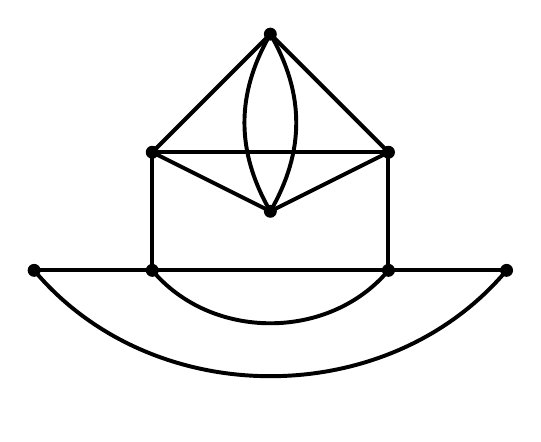
\begin{tikzpicture}[scale=1.5]
	\draw[line width=0.05cm] (-2,0) to (2,0);
	\draw[line width=0.05cm] (-1,0) to (-1,1);
	\draw[line width=0.05cm] (1,0) to (1,1);
	\draw[line width=0.05cm] (-1,1) to (1,1);
	\draw[line width=0.05cm] (-1,1) to (0,2);
	\draw[line width=0.05cm] (1,1) to (0,2);
	\draw[line width=0.05cm] (-1,1) to (0,0.5);
	\draw[line width=0.05cm] (1,1) to (0,0.5);
	\draw[line width=0.05cm, bend right=50] (-1,0) to (1,0);
	\draw[line width=0.05cm, bend right=50] (-2,0) to (2,0);
	\draw[line width=0.05cm, bend right= 30] (0,2) to (0,0.5);
	\draw[line width=0.05cm, bend left= 30] (0,2) to (0,0.5);
	
	\draw[fill= black] (0,2) circle (0.05);
	\draw[fill= black] (-1,1) circle (0.05);
	\draw[fill= black] (1,1) circle (0.05);
	\draw[fill= black] (0,0.5) circle (0.05);
	\draw[fill= black] (-2,0) circle (0.05);
	\draw[fill= black] (-1,0) circle (0.05);
	\draw[fill= black] (1,0) circle (0.05);
	\draw[fill= black] (2,0) circle (0.05);
	\end{tikzpicture}
	\]
\begin{enumerate}[(a)]
\item Does $G$ have an Euler trail? If it does, find it. If it does not, explain why. 
\item Does $G$ have a Hamiltonian circuit? If it does, find it. If it does not, explain why. 
\end{enumerate}





\newpage



% Problem 3
\problem{10} Suppose $G$ is the graph given below on the left and that $H$ is a directed graph with adjacency matrix $A$. Showing all your work and fully justifying your responses, answer the questions below. \par
	\begin{minipage}[c]{0.49\textwidth}
	\[
	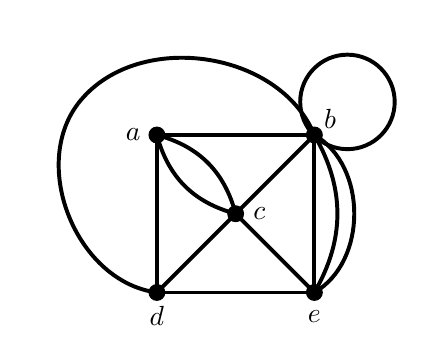
\begin{tikzpicture}[scale=2]
	\draw[line width=0.05cm] (0,0) to (1,0);
	\draw[line width=0.05cm] (0,0) to (0,1);
	\draw[line width=0.05cm] (0,1) to (1,1);
	\draw[line width=0.05cm] (1,0) to (1,1);
	\draw[line width=0.05cm] (0,0) to (1,1);
	\draw[line width=0.05cm] (0.5,0.5) to (1,0);
	\draw[line width=0.05cm, bend right= 30] (0,1) to (0.5,0.5);
	\draw[line width=0.05cm, bend left= 30] (0,1) to (0.5,0.5);
	\draw[line width=0.05cm, bend right= 30] (1,0) to (1,1);
	\draw[line width=0.05cm, bend right= 60] (1,0) to (1,1);
	\draw[line width=0.05cm, bend left= 60] (0,0) to (-0.5,1.2);
	\draw[line width=0.05cm, bend right= 60] (1,1) to (-0.5,1.2);
	\draw[line width=0.05cm] (1.21,1.21) circle (0.3);
	
	\draw[fill= black] (0,0) circle (0.05);
	\draw[fill= black] (1,0) circle (0.05);
	\draw[fill= black] (1,1) circle (0.05);
	\draw[fill= black] (0,1) circle (0.05);
	\draw[fill= black] (0.5,0.5) circle (0.05);
	
	\node at (-0.15,1) {$a$};
	\node at (1.10,1.10) {$b$};
	\node at (0.65,0.50) {$c$};
	\node at (0,-0.15) {$d$};
	\node at (1,-0.15) {$e$};
	\end{tikzpicture}
	\]
	\end{minipage}%
	\begin{minipage}[c]{0.49\textwidth}
	\[
	A^8= 
	\begin{pmatrix}
	408 628 & 1456983 & 1201872 & 1045608 \\
	217055 & 774044 & 638429 & 555540 \\
	442957 & 1577690 & 1299626 & 1131303 \\
	280444 & 1001303 & 825067 & 716683
	\end{pmatrix}
	\]
	\end{minipage}

\begin{enumerate}[(a)]
\item How many walks are there of length 1 from $b$ to $e$? What about from $d$ to $b$?
\item How many walks are there of length 2 from $c$ to itself? What about from $e$ to $a$?
\item How many walks are there of length 4 from $a$ to $c$? What about from $b$ to itself?
\item How many connected components does $G$ have?
\item How many walks are there of length 8 from $v_1$ to $v_3$ in $H$? What about $v_4$ to $v_2$?
\end{enumerate}



\newpage



% Problem 4
\problem{10} Suppose that $G$ is an undirected graph with adjacency matrix, $A$, given below. 
	\[
	A= 
	\begin{pmatrix}
	0 & 2 & 1 & 0 & 0 & 0 & 0 & 0 \\
	2 & 0 & 1 & 0 & 0 & 0 & 0 & 0 \\
	1 & 1 & 0 & 0 & 0 & 0 & 0 & 0 \\
	0 & 0 & 0 & 0 & 1 & 0 & 0 & 0 \\
	0 & 0 & 0 & 1 & 1 & 2 & 0 & 0 \\
	0 & 0 & 0 & 0 & 2 & 0 & 0 & 0 \\
	0 & 0 & 0 & 0 & 0 & 0 & 0 & 0 \\
	0 & 0 & 0 & 0 & 0 & 0 & 0 & 1
	\end{pmatrix}
	\]
Using only this adjacency matrix, showing all your work, fully justifying your responses, answer the following:
\begin{enumerate}[(a)]
\item Is $G$ a simple graph?
\item Is $G$ a multigraph?
\item How many connected components does $G$ have?
\item Find the degrees of vertices $v_1$, $v_8$, and $v_5$.
\item What is the degree of $G$?
\end{enumerate}


\end{document}